\documentclass[12pt]{article}
\usepackage{amsmath,amsthm,amssymb,hyperref,fancyhdr,color,multicol,enumitem}
\usepackage[margin=.5in,bottom=1in]{geometry}
\usepackage{pgfplots}
\pgfplotsset{compat=1.11}

\newcommand{\R}{\mathbb{R}}
\newcommand{\Z}{\mathbb{Z}}

\pagestyle{fancy} 
\fancyhf{}\renewcommand{\headrulewidth}{0pt}

\newcommand{\graphA}{
	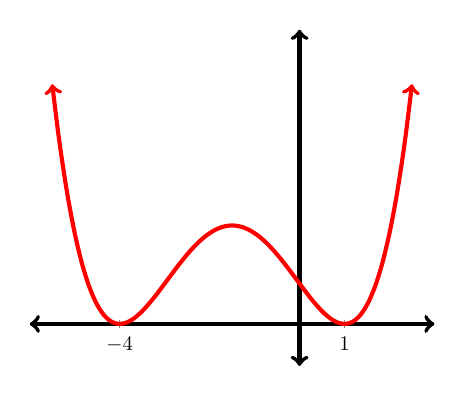
\begin{tikzpicture}[scale=.75]
		\begin{axis}[ 
		axis lines = middle,
		axis line style={<->},
		xmin=-6, xmax=3,
		ymin=-100, ymax=700,
		grid=none,
		xtick={-4,1},
		ytick=\empty,
		samples=50,
		smooth,
		no markers,
		domain=-5.5:2.5,
		line width=2pt
		]
		\addplot[<->,red] {6*(x+4)^2*(x-1)^2};
		\end{axis}
	\end{tikzpicture}
}
\newcommand{\graphB}{
	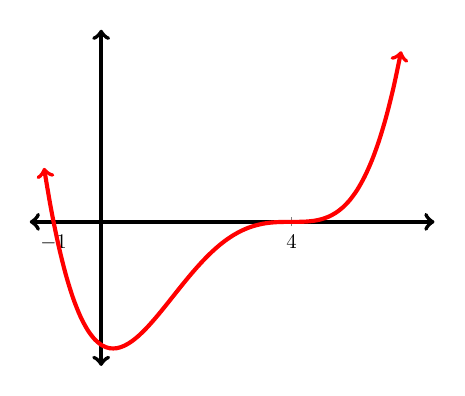
\begin{tikzpicture}[scale=.75]
		\begin{axis}[ 
		axis lines = middle,
		axis line style={<->},
		xmin=-1.5, xmax=7,
		ymin=-600, ymax=800,
		grid=none,
		%ticklabel style=left,
		xtick={4,-1},
		ytick=\empty,
		samples=50,
		smooth,
		no markers,
		domain=-1.2:6.3,
		line width=2pt
		]
		\addplot[<->,red] {8*(x-4)^3*(x+1)};
		\end{axis}
	\end{tikzpicture}
}
\newcommand{\graphC}{	
	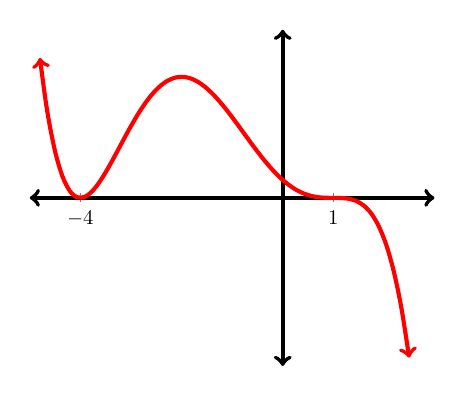
\begin{tikzpicture}[scale=.75]
		\begin{axis}[ 
			axis lines = middle,
			axis line style={<->},
			xmin=-5, xmax=3,
			ymin=-450, ymax=450,
			grid=none,
			xtick={-4,1},
			ytick=\empty,
			samples=50,
			smooth,
			no markers,
			domain=-4.8:2.5,
			line width=2pt
			]
			\addplot[<->,red] {-3*(x+4)^2*(x-1)^3};
		\end{axis}
	\end{tikzpicture}
}
\newcommand{\graphD}{
		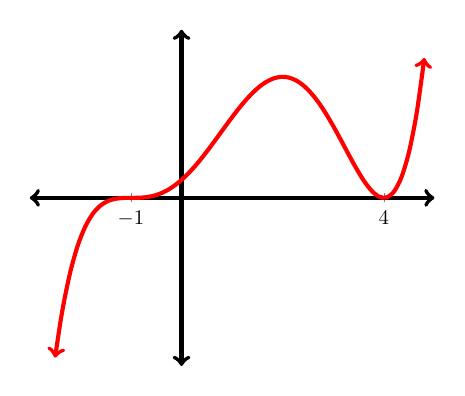
\begin{tikzpicture}[scale=.75]
		\begin{axis}[ 
			axis lines = middle,
			axis line style={<->},
			xmin=-3, xmax=5,
			ymin=-300, ymax=300,
			grid=none,
			xtick={4,-1},
			ytick=\empty,
			samples=50,
			smooth,
			no markers,
			domain=-2.5:4.8,
			line width=2pt
			]
			\addplot[<->,red] {2*(x-4)^2*(x+1)^3};
		\end{axis}
	\end{tikzpicture}
}
\newcommand{\graphE}{
	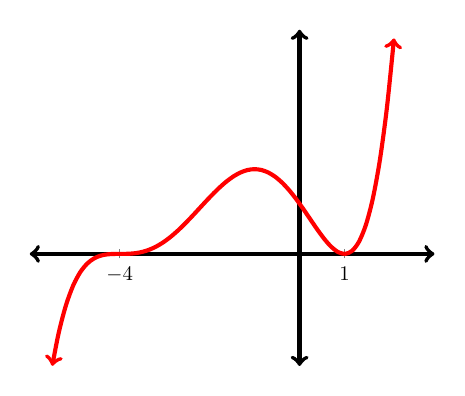
\begin{tikzpicture}[scale=.75]
		\begin{axis}[ 
			axis lines = middle,
			axis line style={<->},
			xmin=-6, xmax=3,
			ymin=-1000, ymax=2000,
			grid=none,
			xtick={-4,1},
			ytick=\empty,
			samples=50,
			smooth,
			no markers,
			domain=-5.5:2.1,
			line width=2pt
			]
			\addplot[<->,red] {7*(x+4)^3*(x-1)^2};
		\end{axis}
	\end{tikzpicture}
}
\newcommand{\graphF}{
		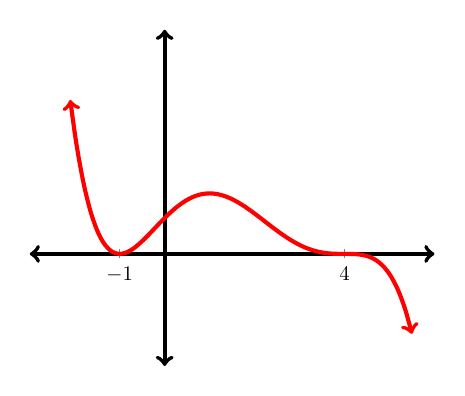
\begin{tikzpicture}[scale=.75]
		\begin{axis}[ 
			axis lines = middle,
			axis line style={<->},
			xmin=-3, xmax=6,
			ymin=-1000, ymax=2000,
			grid=none,
			xtick={4,-1},
			ytick=\empty,
			samples=50,
			smooth,
			no markers,
			domain=-2.1:5.5,
			line width=2pt
			]
			\addplot[<->,red] {-5*(x-4)^3*(x+1)^2};
		\end{axis}
	\end{tikzpicture}
}

\begin{document}
	\noindent Math 109: Algebra for Calculus\hfill Exam 4 Review\\
	\mbox{}\hfill Chapter 4: Exponential and Logarithmic Functions
	\setcounter{page}{1}
	\fancyfoot[C]{\thepage}
\begin{enumerate}
	
	%4.1
	\item Sketch a graph of the functions then determine if they are invertible (aka are they one-to-one?)
		\begin{enumerate}
			\item $f(x)=x^3-1$\vfill
			\item $g(x)=2x^2+1$\vfill
		\end{enumerate}
	\item Are the functions $m(x)=\sqrt[3]{x+1}$ and $n(x)=(x-1)^3$ inverses?\vfill
	\item Write an equation for the inverse function.
		\begin{enumerate}
			\item $f(x)=2x^3-5$\vfill
			\item $g(x)=\dfrac{2}{x+7}$\vfill
		\end{enumerate}
	
	
	
	%4.2
	\newpage
	\item Sketch a graph of the function $f(x)=\left(\dfrac{10}{3}\right)^x$.\vfill
	\item What are the transformations we should apply to the graph of $y=3^x$ to get a graph of $y=-3^x+1$.  (Note that order is going to be important here so make sure to check you got that right.)
	\vfill
	\newpage
	\item The population of Canada in 2010 was approximately 34 million with an annual growth rate of $0.804\%$.  At this rate, the population $P(t)$ (in millions) can be approximated by 
	$$P(t)=34(1.00804)^t$$ where $t$ is the time in years since 2010.
		\begin{enumerate}
			\item Is the graph of $p$ increasing or decreasing? Why?\vskip 1in
			\item Evaluate $P(0)$ and interpret its meaning in the context of this problem.\vfill
			\item Evaluate $P(5)$ and interpret its meaning in the context of this problem. Round the population value to the nearest million.\vfill
			\item Evaluate $P(13)$ then check online for the actual current population of Canada.  How accurate is this model?\vfill
		\end{enumerate}
	
	
	
	%4.3
	\newpage
	\item Write in exponential form
		\begin{multicols}{2}
			\begin{enumerate}
				\item $\log_b(x^2+y^2)=4$
				\item $\ln x=c+d$
			\end{enumerate}
		\end{multicols}
		\vfill
	\item Write in logarithmic form
		\begin{multicols}{2}
			\begin{enumerate}
				\item $10^{xy}=5c$
				\item $8^{-1/3}=\frac{1}{2}$
			\end{enumerate}
		\end{multicols}
		\vfill
	\item Let $h(x)=\log(x-3)$.
		\begin{enumerate}
			\item Write the domain in interval notation.
			\vfill
			\item Write the range in interval notation.
			\vfill
			\item Write an equation for the vertical asymptote.
			\vfill
			\item Sketch a graph of the function.
			\vfill
			\vfill
		\end{enumerate}
	\newpage
	\item Let $h(x)=2+\ln(x)$.
		\begin{enumerate}
			\item Write the domain in interval notation.
			\vfill
			\item Write the range in interval notation.
			\vfill
			\item Write an equation for the vertical asymptote.
			\vfill
			\item Sketch a graph of the function.
			\vfill
			\vfill
		\end{enumerate}
	\newpage
	
	
	
	%4.4
	\newpage
	\item Expand and simplify
		\begin{enumerate}
			\item $\log_2\left(\dfrac{1}{8}a^2b\right)$\vfill
			\item $\log\left(\dfrac{x^2(2x+1)^5}{\sqrt{1-x}}\right)$\vfill
		\end{enumerate}
	\item If $\ln(a)=5$, $\ln(b)=2$, and $\ln(c)=7$, compute $\ln\left(\dfrac{\sqrt[3]{ab^2}}{c^3}\right)$.
		\vfill
	\newpage
	\item Write as a single logarithm
		\begin{enumerate}
			\item $4\log_5(y)-3\log_5(x)+\dfrac{1}{2}\log_5(z)$\vfill
			\item $\log(250)+\log(2)-\log(5)$\vfill
			\item $\dfrac{1}{4}\ln(x^2-9)-\dfrac{1}{4}\ln(x-3)$\vfill
		\end{enumerate}
	\item Write $\log\left(xy^2\sqrt{x^3y^4\sqrt{x^5y^6}}\right)$ as $A\log(x)+B\log(y)$.
		\vfill
	
	
	
	% 4.5
	\newpage
	\item Solve the equation
		\begin{enumerate}
			\item $1000^{2x+1}=\left(\dfrac{1}{100}\right)^{x-4}$\vfill
			\item $2^{c+3}=7^{2c+5}$\vfill
			\item $2(10^{1.2t})=58$\vfill
			\item $\log_5(4p+7)=\log_5(2-p)$\vfill
			\item $2\log_6(4-8y)+6=10$\vfill
			\item $\ln x+\ln(x+2)=\ln(x+6)$\vfill
		\end{enumerate}
	\newpage
	\item Suppose that \$50,000 is invested in an account that earns $7\%$ interest per year compounded monthly.
		\begin{enumerate}
			\item What is the account balance after 5 years?\vfill
			\item How many years will it take for the account balance to reach \$75,000?\vfill
		\end{enumerate}
	
	\item Caffeine occurs naturally in a variety of food products such as coffee, tea, and chocolate. The kidneys filter the blood and remove caffeine.  The biological half-life of caffeine is approximately 6 hr. 
	%If one cup of coffee has 80 mg of caffeine, then the amount of caffeine $C$ (in mg) remaining after $t$ hours is given by $C=80(2^{-t/6})$.
		\begin{enumerate}
			\item If we drink a cup of coffee with 80 mg of caffeine, how long will it take for the amount of caffeine to drop below 60 mg? Round to 1 decimal place.\vfill
			\item Laura has trouble sleeping if she has more than 30 mg of caffeine in her bloodstream. How many hours after drinking coffee would Laura have to wait so that the coffee would not disrupt her sleep? Round to 1 decimal place.\vfill
		\end{enumerate}
	
	
	
	% 4.6
	\newpage
	\item The population of a certain region is growing exponentially. There were 35 million people on January 1, 1980 and 80 million people on January 1, 1990.
	
		\begin{enumerate}
			\item Find an exponential growth model for the population (in millions of people) at any time $t$ in years after 1980.
			\vfill
			\item What population do you predict for the year 2000?
			\vfill
			\item How many years does it take for the population to double?
			\vfill
		\end{enumerate}
	
	
	
	%Summary	
	\newpage
	\item For each Section in Chapter 4, write down the key terms and ideas.
	\begin{enumerate}
		\item Section 4.1: \vfill
		\item Section 4.2: \vfill
		\item Section 4.3: \vfill
		\newpage
		\item Section 4.4: \vfill
		\item Section 4.5: \vfill 
		\item Section 4.6: \vfill 
	\end{enumerate}
\end{enumerate}
\end{document}